\documentclass[slideopt,A4,showboxes,svgnames]{beamer}

%% list of packages here
\usepackage[absolute,showboxes,overlay]{textpos}
\usepackage{booktabs}
\usepackage{mathtools}
\usepackage{amsmath}
\usepackage{amssymb}
\usepackage{pifont}
\usepackage{multicol}
\usepackage{multirow}
\usepackage{array, makecell}
\usepackage{blkarray}
\usepackage[linesnumbered,ruled,vlined]{algorithm2e}
\usepackage[backend=biber, style=authoryear]{biblatex}
\renewcommand*{\nameyeardelim}{\addcomma\addspace}
\addbibresource{../references.bib}

\usepackage{theme/beamerthemeinria}


%%%%%%%%%%%%%%%%%%%%%%%%%%%%
% Paper dependent stuff    %
%%%%%%%%%%%%%%%%%%%%%%%%%%%%

\newcommand{\Tau}{T}

\newcommand{\hlrb}[1]{\bm{\textcolor{Red}{#1}}}
\newcommand{\hlbb}[1]{\bm{\textcolor{Blue}{#1}}}
\newcommand{\hlgb}[1]{\bm{\textcolor{Green}{#1}}}

\newcommand{\OPD}{\texttt{OPD}}

%%%%%%%%%%%%%%%%%%%%%%%%%%%%
% Aesthetics               %
% over-underline, hat, bold%
%%%%%%%%%%%%%%%%%%%%%%%%%%%%

\newcommand{\eps}{\varepsilon}
\newcommand{\vareps}{\varepsilon}
\renewcommand{\epsilon}{\varepsilon}
%\renewcommand{\hat}{\widehat}
\renewcommand{\tilde}{\widetilde}
\renewcommand{\bar}{\overline}

\newcommand*{\MyDef}{\mathrm{\tiny def}}
\newcommand*{\eqdefU}{\ensuremath{\mathop{\overset{\MyDef}{=}}}}% Unscaled version
% \newcommand*{\eqdef}{\mathop{\overset{\MyDef}{\resizebox{\widthof{\eqdefU}}{\heightof{=}}{=}}}}
\newcommand{\eqdef}{\stackrel{def}{=}}


\def\:#1{\protect \ifmmode {\mathbf{#1}} \else {\textbf{#1}} \fi}
\newcommand{\CommaBin}{\mathbin{\raisebox{0.5ex}{,}}}

\newcommand{\wt}[1]{\widetilde{#1}}
\newcommand{\wh}[1]{\widehat{#1}}
\newcommand{\wo}[1]{\overline{#1}}
\newcommand{\wb}[1]{\overline{#1}}

% bf and bm missing due to conflict!!
\newcommand{\bsym}[1]{\mathbf{#1}}
\newcommand{\bzero}{\mathbf{0}}
\newcommand{\ba}{\mathbf{a}}
\newcommand{\bb}{\mathbf{b}}
\newcommand{\bc}{\mathbf{c}}
\newcommand{\bd}{\mathbf{d}}
\newcommand{\be}{\mathbf{e}}
\newcommand{\bg}{\mathbf{g}}
\newcommand{\bh}{\mathbf{h}}
\newcommand{\bi}{\mathbf{i}}
\newcommand{\bj}{\mathbf{j}}
\newcommand{\bk}{\mathbf{k}}
\newcommand{\bl}{\mathbf{l}}
\newcommand{\bn}{\mathbf{n}}
\newcommand{\bo}{\mathbf{o}}
\newcommand{\bp}{\mathbf{p}}
\newcommand{\bq}{\mathbf{q}}
\newcommand{\br}{\mathbf{r}}
\newcommand{\bs}{\mathbf{s}}
\newcommand{\bt}{\mathbf{t}}
\newcommand{\bu}{\mathbf{u}}
\newcommand{\bv}{\mathbf{v}}
\newcommand{\bw}{\mathbf{w}}
\newcommand{\bx}{\mathbf{x}}
\newcommand{\by}{\mathbf{y}}
\newcommand{\bz}{\mathbf{z}}

\newcommand{\bA}{\mathbf{A}}
\newcommand{\bB}{\mathbf{B}}
\newcommand{\bC}{\mathbf{C}}
\newcommand{\bD}{\mathbf{D}}
\newcommand{\bE}{\mathbf{E}}
\newcommand{\bF}{\mathbf{F}}
\newcommand{\bG}{\mathbf{G}}
\newcommand{\bH}{\mathbf{H}}
\newcommand{\bI}{\mathbf{I}}
\newcommand{\bJ}{\mathbf{J}}
\newcommand{\bK}{\mathbf{K}}
\newcommand{\bL}{\mathbf{L}}
\newcommand{\bM}{\mathbf{M}}
\newcommand{\bN}{\mathbf{N}}
\newcommand{\bO}{\mathbf{O}}
\newcommand{\bP}{\mathbf{P}}
\newcommand{\bQ}{\mathbf{Q}}
\newcommand{\bR}{\mathbf{R}}
\newcommand{\bS}{\mathbf{S}}
\newcommand{\bT}{\mathbf{T}}
\newcommand{\bU}{\mathbf{U}}
\newcommand{\bV}{\mathbf{V}}
\newcommand{\bW}{\mathbf{W}}
\newcommand{\bX}{\mathbf{X}}
\newcommand{\bY}{\mathbf{Y}}
\newcommand{\bZ}{\mathbf{Z}}

% calligraphic
\newcommand{\cf}{\mathcal{f}}
\newcommand{\cA}{\mathcal{A}}
\newcommand{\cB}{\mathcal{B}}
\newcommand{\cC}{\mathcal{C}}
\newcommand{\cD}{\mathcal{D}}
\newcommand{\cE}{\mathcal{E}}
\newcommand{\cF}{\mathcal{F}}
\newcommand{\cG}{\mathcal{G}}
\newcommand{\cH}{\mathcal{H}}
\newcommand{\cI}{\mathcal{I}}
\newcommand{\cJ}{\mathcal{J}}
\newcommand{\cK}{\mathcal{K}}
\newcommand{\cL}{\mathcal{L}}
\newcommand{\cM}{\mathcal{M}}
\newcommand{\cN}{\mathcal{N}}
\newcommand{\cO}{\mathcal{O}}
\newcommand{\cP}{\mathcal{P}}
\newcommand{\cQ}{\mathcal{Q}}
\newcommand{\cR}{\mathcal{R}}
\newcommand{\cS}{\mathcal{S}}
\newcommand{\cT}{\mathcal{T}}
\newcommand{\cU}{\mathcal{U}}
\newcommand{\cV}{\mathcal{V}}
\newcommand{\cW}{\mathcal{W}}
\newcommand{\cX}{\mathcal{X}}
\newcommand{\cY}{\mathcal{Y}}
\newcommand{\cZ}{\mathcal{Z}}

%%%%%%%%%%%%%%%%%%%%%%%%%%%%
% Math jargon              %
%%%%%%%%%%%%%%%%%%%%%%%%%%%%
\newcommand{\wrt}{w.r.t.\xspace}
\newcommand{\defeq}{\stackrel{\mathclap{\normalfont\mbox{\tiny def}}}{=}}
\newcommand{\maxund}[1]{\max\limits_{#1}}
\newcommand{\supund}[1]{\text{sup}\limits_{#1}}
\newcommand{\minund}[1]{\min\limits_{#1}}
\renewcommand{\epsilon}{\varepsilon}
\newcommand{\bigotime}{\mathcal{O}}


\DeclareMathOperator*{\argmin}{arg\,min} 
\DeclareMathOperator*{\argmax}{arg\,max} 
\DeclareMathOperator*{\cupdot}{\mathbin{\mathaccent\cdot\cup}}

%%%%%%%%%%%%%%%%%%%%%%%%%%%%
% Matrix operators         %
%%%%%%%%%%%%%%%%%%%%%%%%%%%%
\newcommand{\transpose}{^\mathsf{\scriptscriptstyle T}}
\newcommand{\transp}{\mathsf{\scriptscriptstyle T}}

%%%%%%%%%%%%%%%%%%%%%%%%%%%%
% Statistic operators      %
%%%%%%%%%%%%%%%%%%%%%%%%%%%%
\newcommand{\probability}[1]{\mathbb{P}\left(#1\right)}
\newcommand{\probdist}{Pr}
\DeclareMathOperator*{\expectedvalue}{\mathbb{E}}
\DeclareMathOperator*{\variance}{\text{Var}}
\newcommand{\expectedvalueover}[1]{\expectedvalue\limits_{#1}}
\newcommand{\condbar}{\;\middle|\;}
\newcommand{\gaussdistr}{\mathcal{N}}
\newcommand{\uniformdistr}{\mathcal{U}}
\newcommand{\bernoullidist}{\mathcal{B}}

%%%%%%%%%%%%%%%%%%%%%%%%%%%%
% Algebraic Sets           %
%%%%%%%%%%%%%%%%%%%%%%%%%%%%
\newcommand{\Real}{\mathbb{R}}
\newcommand{\Natural}{\mathbb{N}}
\newcommand{\statespace}{\mathcal{X}}
\newcommand{\funcspace}{\mathcal{F}}
\newcommand{\dynaspace}{\mathcal{T}}

%
%\newtheorem{theorem}{Theorem}
%\newtheorem{definition}{Definition}
%\newtheorem{lemma}{Lemma}
%\providecommand*\lemmaautorefname{Lemma}
%\newtheorem{proposition}{Proposition}
%\providecommand*\propositionautorefname{Proposition}
%\newtheorem{remark}{Remark}
%\newtheorem{property}{Property}
%\newtheorem{assumption}{Assumption}
%\providecommand*\assumptionautorefname{Assumption}
%\newtheorem{conjecture}{Conjecture}
\providecommand*\algorithmautorefname{Algorithm}

\addto\extrasenglish{  
	\def\algorithmautorefname{Algorithm}  
}
%
%\newtheorem*{definition*}{Definition}
%\newtheorem*{theorem*}{Theorem}
%\newtheorem*{proposition*}{Proposition}
%\newtheorem*{remark*}{Remark}

% Colors for slides
\definecolor{rouge1}{RGB}{226,0,38}  % red P
\definecolor{orange1}{RGB}{243,154,38}  % orange P
\definecolor{jaune}{RGB}{254,205,27}  % jaune P
\definecolor{blanc}{RGB}{255,255,255} % blanc P

\definecolor{rouge2}{RGB}{230,68,57}  % red S
\definecolor{orange2}{RGB}{236,117,40}  % orange S
\definecolor{taupe}{RGB}{134,113,127} % taupe S
\definecolor{gris}{RGB}{91,94,111} % gris S
\definecolor{bleu1}{RGB}{38,109,131} % bleu S
\definecolor{bleu2}{RGB}{28,50,114} % bleu S
\definecolor{vert1}{RGB}{133,146,66} % vert S
\definecolor{vert3}{RGB}{20,200,66} % vert S
\definecolor{vert2}{RGB}{157,193,7} % vert S
\definecolor{vertsolarized}{RGB}{211,233,219} % vert S
\definecolor{darkyellow}{RGB}{233,165,0}  % orange S
\definecolor{lightgray}{rgb}{0.9,0.9,0.9}
\definecolor{darkgray}{rgb}{0.6,0.6,0.6}

\newcommand{\incarrow}{{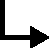
\includegraphics[height=0.7\baselineskip]{./theme/img/arrow_list}}}


% Highlights for slides
\newcommand{\rcol}[1]{\textcolor{red}{\textit{#1}}}
%\newcommand{\eqrcol}[1]{\textcolor{red}{#1}}
%\newcommand{\eqrcolb}[1]{\textcolor{red}{\boldsymbol{#1}}}
\newcommand{\gcol}[1]{\textcolor{vert3}{\textit{#1}}}
%\newcommand{\eqgcol}[1]{\textcolor{vert3}{#1}}
%\newcommand{\eqgcolb}[1]{\textcolor{vert3}{\boldsymbol{#1}}}
\newcommand{\blcol}[1]{\textcolor{blue}{\textit{#1}}}
%\newcommand{\eqbcol}[1]{\textcolor{blue}{#1}}
%\newcommand{\eqbcolb}[1]{\textcolor{blue}{\boldsymbol{#1}}}
\newcommand{\ycol}[1]{\textcolor{darkyellow}{\textit{#1}}}
\newcommand{\eqycol}[1]{\textcolor{darkyellow}{#1}}

\newcommand{\rcolbm}[1]{$\textcolor{red}{\boldsymbol{#1}}$}
\newcommand{\rcolb}[1]{\textcolor{red}{\textit{\textbf{#1}}}}
\newcommand{\gcolb}[1]{\textcolor{vert3}{\textit{\textbf{#1}}}}
\newcommand{\bcolb}[1]{\textcolor{blue}{\textit{\textbf{#1}}}}
\newcommand{\ycolb}[1]{\textcolor{darkyellow}{\textit{\textbf{#1}}}}

% Colored boxes
\newcounter{ColoredBoxesCounter}
\newcommand{\highlightnew}[3][(0.0,-0.1)(-0.0,0.3)]{
\hfsetfillcolor{#2!20}
\hfsetbordercolor{#2!80}
\tikzmarkin{\theColoredBoxesCounter}#1
#3
\tikzmarkend{\theColoredBoxesCounter}
\stepcounter{ColoredBoxesCounter}
}

\newcommand{\highlight}[2][yellow]{\mathchoice%
{\colorbox{#1}{$\displaystyle#2$}}%
{\colorbox{#1}{$\textstyle#2$}}%
{\colorbox{#1}{$\scriptstyle#2$}}%
{\colorbox{#1}{$\scriptscriptstyle#2$}}}%

\newcommand{\eqrcol}[1]{\highlight[red!20]{#1}}
\newcommand{\eqrcolb}[1]{\highlight[red!20]{\boldsymbol{#1}}}
\newcommand{\eqgcol}[1]{\highlight[vert3!20]{#1}}
\newcommand{\eqgcolb}[1]{\highlight[vert3!20]{\boldsymbol{#1}}}
\newcommand{\eqbcol}[1]{\highlight[blue!20]{#1}}
\newcommand{\eqbcolb}[1]{\highlight[blue!20]{\boldsymbol{#1}}}

\colorlet{redp}{red!20} % vert S
\colorlet{greenp}{vert3!20} % vert S
\colorlet{bluep}{blue!20} % vert S
\colorlet{yellowp}{yellow!20} % vert S

\usepackage{soul}
\renewcommand{\hl}[3][\fboxsep1pt]{{#1\colorbox{#2}{#3}}}%

\newcommand{\hlr}[1]{\hl{redp}{#1}}
\newcommand{\hlg}[1]{\hl{greenp}{#1}}
\newcommand{\hlb}[1]{\hl{bluep}{#1}}
\newcommand{\hly}[1]{\hl{yellowp}{#1}}

\newcommand{\hler}[1]{\hl[\fboxsep0pt]{redp}{$\displaystyle {#1}$}}
\newcommand{\hleg}[1]{\hl[\fboxsep0pt]{greenp}{$\displaystyle {#1}$}}
\newcommand{\hleb}[1]{\hl[\fboxsep0pt]{bluep}{$\displaystyle {#1}$}}

\newcommand{\hlbr}[1]{\hl[\fboxsep0pt]{redp}{$\displaystyle \mathbf{#1}$}}
\newcommand{\hlbg}[1]{\hl[\fboxsep0pt]{greenp}{$\displaystyle \mathbf{#1}$}}
\newcommand{\hlbb}[1]{\hl[\fboxsep0pt]{bluep}{$\displaystyle \mathbf{#1}$}}

\newcommand{\vph}{\vphantom{A_A^A}}

% Box for algorithms
\newlength{\minipagewidth}
\newlength{\minipagewidthx}
\setlength{\minipagewidth}{\columnwidth}
\setlength{\minipagewidthx}{\columnwidth}
\setlength{\fboxsep}{0.1mm}
\addtolength{\minipagewidth}{-\fboxrule}
\addtolength{\minipagewidth}{-\fboxrule}
\addtolength{\minipagewidth}{-\fboxsep}
\addtolength{\minipagewidth}{-\fboxsep}
\addtolength{\minipagewidthx}{+\fboxsep}
\newcommand{\bookbox}[1]{\small
\par\medskip\noindent
\framebox[\columnwidth]{
\begin{minipage}{\minipagewidth} {#1} \end{minipage} } \par\medskip }

\newcommand{\bookboxx}[1]{
\par\medskip\noindent
\framebox[\columnwidth]{
\begin{minipage}[t]{0.98\columnwidth} {\par\smallskip#1\par\smallskip} \end{minipage} } \par\medskip }


\usepackage{array}
\newcolumntype{L}[1]{>{\raggedright\let\newline\\\arraybackslash\hspace{-3.1cm}}m{#1}}
\newcolumntype{C}[1]{>{\centering\let\newline\\\arraybackslash\hspace{135pt}}m{#1}}
\newcolumntype{R}[1]{>{\raggedleft\let\newline\\\arraybackslash\hspace{-10pt}}m{#1}}

\newenvironment{myfont}{\fontfamily{kurier}\selectfont}{\par}
\newenvironment{myfont2}{\fontfamily{epigrafica}\selectfont}{\par}

% Border color of content boxes
\definecolor{bordercol}{RGB}{0,0,0}  %black
% Background color for the header in the content boxes (left side)
\definecolor{headercol1}{RGB}{200,0,0}        %red:RGB {200,0,0} 
% Background color for the header in the content boxes (right side) 
\definecolor{headercol2}{rgb}{1.0,0.49,0.0}        %orange:rgb {1.0,0.49,0.0}
% Text color for the header text in the content boxes
\definecolor{headerfontcol}{rgb}{1,1,1}  %white
% Background color for the content in the boxes
\definecolor{boxcolor}{rgb}{1,1,1} 

\definecolor{lightblue}{rgb}{0.145,0.6666,1}

\newsavebox\CBox
\newcommand\hcancel[2][0.5pt]{%
  \ifmmode\sbox\CBox{$#2$}\else\sbox\CBox{#2}\fi%
  \makebox[0pt][l]{\usebox\CBox}%  
  \rule[0.3\ht\CBox-#1/2]{\wd\CBox}{#1}}


\title[Monte-Carlo Graph Search]{Monte-Carlo Graph Search:}
\subtitle{the Value of Merging Similar States}
\date[date]{date}
\author[Edouard Leurent]{\textbf{Edouard Leurent}\inst{1,2},\\
	Odalric-Ambrym Maillard\inst{1}}
\institute{
	\inst{1} Univ. Lille, Inria, CNRS, \\ ~Centrale Lille, UMR 9189 – CRIStAL,\\
	\inst{2} Renault Group}

\begin{document}

\begin{frame}
    \titlepage
\end{frame}

\begin{frame}{Motivation}
\begin{alertblock}{Monte-Carlo Tree Search algorithms}
\begin{itemize}[<+->]
	\item rely on a \alert{tree structure} to represent their value estimates.
	\begin{center}
		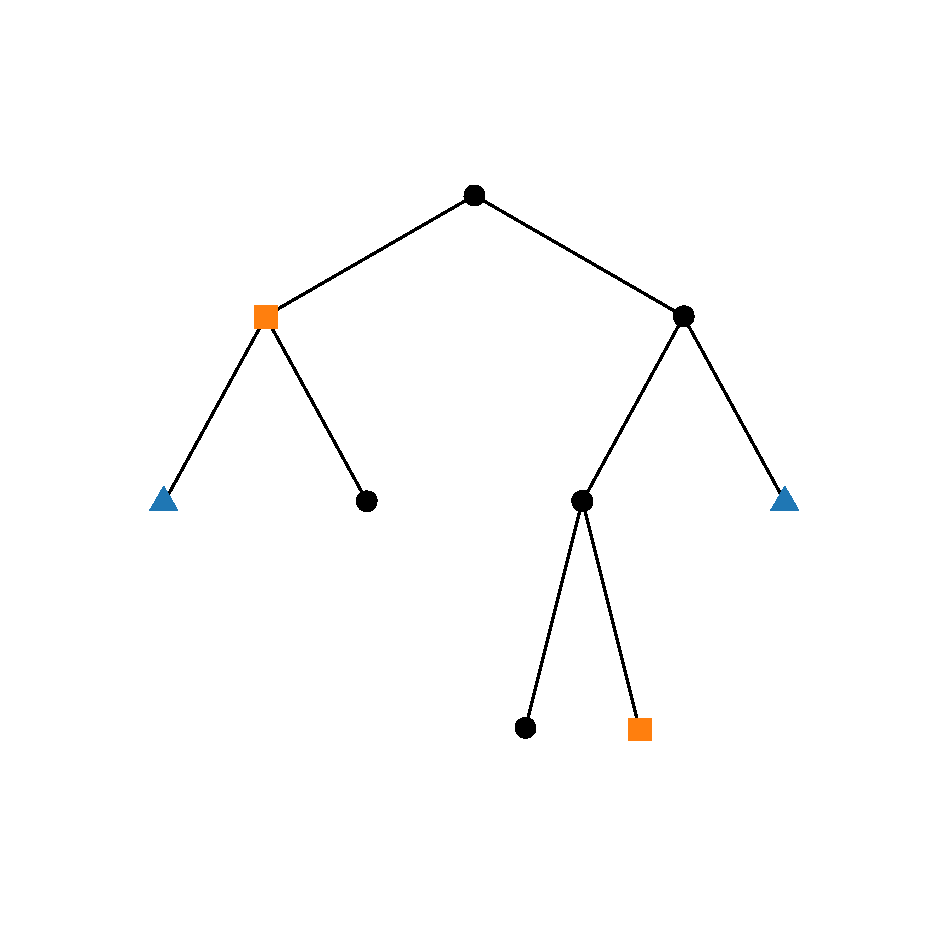
\includegraphics[trim={1.8cm 2.2cm 1.9cm 2.7cm}, clip, width=0.38\linewidth]{img/tree_simple}
	\end{center}
	\item performance {\green independent} of the {\red size $S$ of the state space}%, but with the branching factor $K$ and planning horizon $H$ / budget $n$.
\begin{center}
	\begin{tabular}{lcc}
		Tabular RL & (\texttt{UCBVI}) & $\sqrt{H{\red S}{\green A}n}$ \\
		MCTS & (\texttt{OPD}) & $n^{-\log\frac{1}{\gamma}/\log {\green A}}$
	\end{tabular}
\end{center}
\end{itemize}
\end{alertblock} 
\end{frame}

\begin{frame}{Limitation}
	\begin{itemize}
		\item There can be several paths to the same state {\orange $s$}
		\begin{center}
			\includegraphics<1>[trim={3cm 8cm 3cm 4cm}, clip, width=0.85\linewidth]{img/paths_1}%
			\includegraphics<2>[trim={3cm 8cm 3cm 4cm}, clip, width=0.85\linewidth]{img/paths_2}%
			\includegraphics<3>[trim={3cm 8cm 3cm 4cm}, clip, width=0.85\linewidth]{img/paths_3}%
			\includegraphics<4-6>[trim={3cm 8cm 3cm 4cm}, clip, width=0.85\linewidth]{img/paths_4}%
		\end{center}
		\item<5-6>  {\orange $s$} is represented several times in the tree
		\item<6> {\red No information is shared} between these paths
	\end{itemize}	
\end{frame}

\begin{frame}{Motivating example}
\begin{alertblock}{Not accounting for state similarity hinders exploration}
	\pause
	Sparse gridworld: reward of 0 everywhere
	\begin{center}
	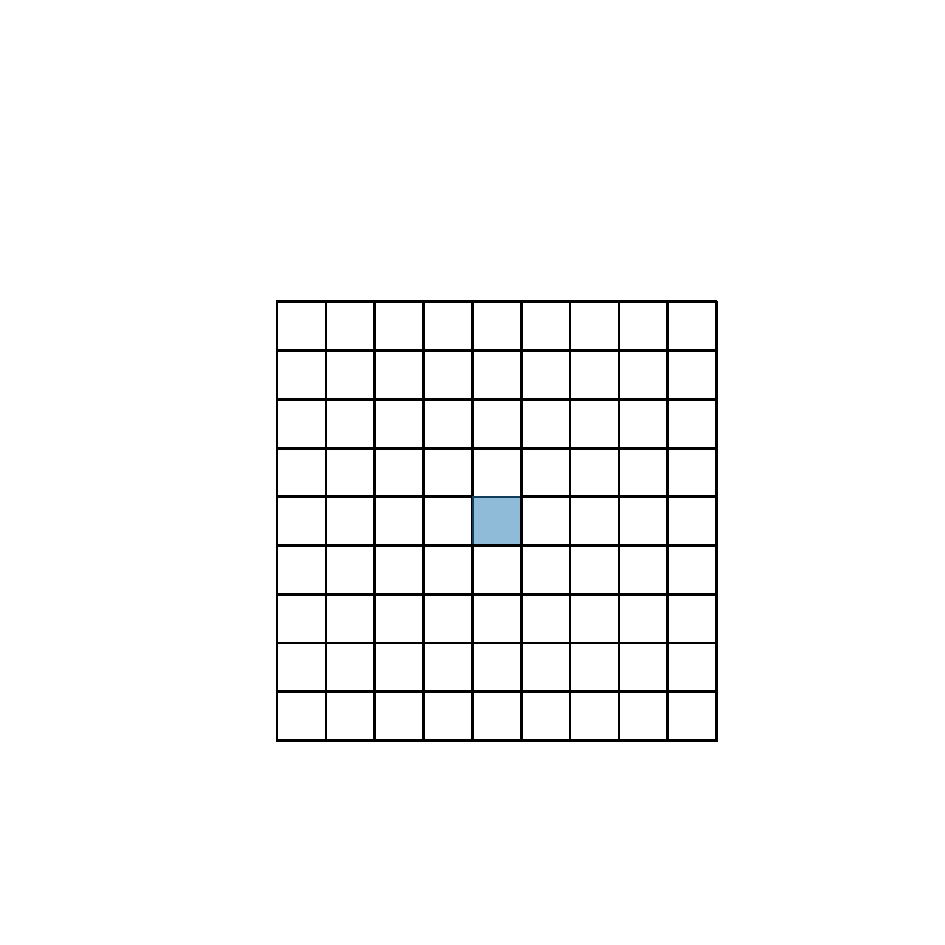
\includegraphics[trim={4cm 3.2cm 3.5cm 4.5cm}, clip, width=0.5\linewidth]{img/sparse_grid}	
	\end{center}
\end{alertblock}
\end{frame}

\begin{frame}{Planners behaviours}
\begin{itemize}
	\item[\incarrow] \alert{Uniform planning} in the space of sequences of actions %  (UCT, OPD, OLOP, etc.) which seems reasonable
\end{itemize}
\begin{center}
	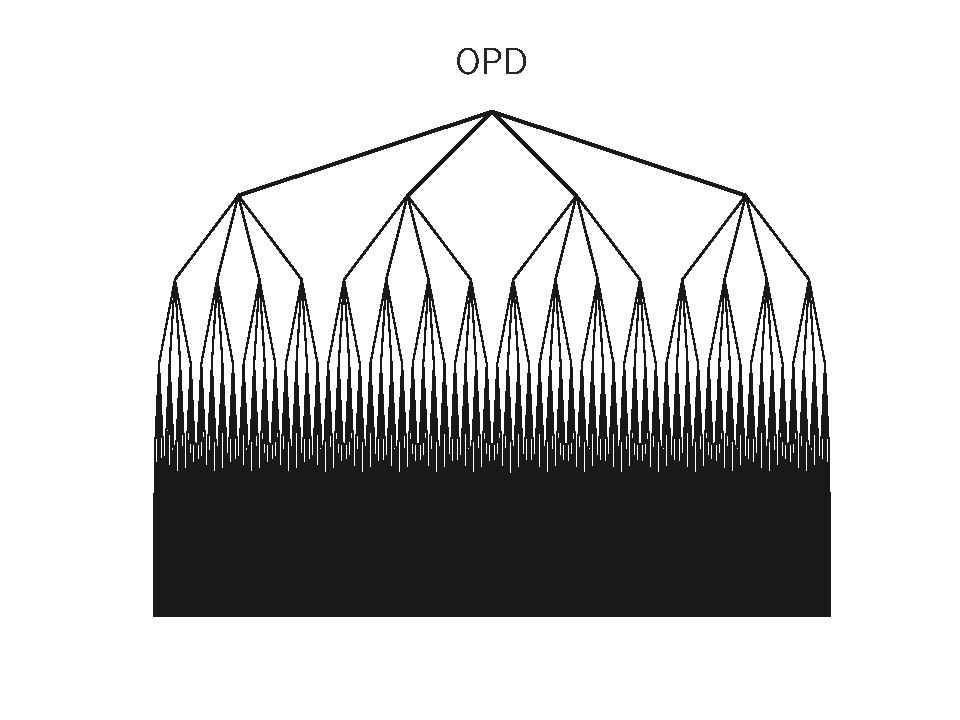
\includegraphics[trim={0 1cm 0 1.5cm},clip,width=0.7\linewidth]{../img/tree_OPD}
	
	\texttt{OPD}, budget of $n=5460$ moves
\end{center}

\end{frame}

\begin{frame}{Motivating example 2/2}
\begin{alertblock}{Concentration}
\begin{itemize}[<+->]
\item Does not lead to uniform exploration of the state space
% but that does not lead to uniform exploration in the state space, because many overlaps between the explored paths
% it spends a lot of time to move mack and forth to states already visited through other trajectories
\item 2D random walk $\sim$ Rayleigh distribution
$P(d) = \frac{2d}{H}e^{-\frac{-d^2}{H}}$
\pause
% similar to random walk: if you sample moves with a uniform distribution, you will not explore far and concentrate around the initial position. Probability to reach a distance d is (1/4)^d

\begin{center}
	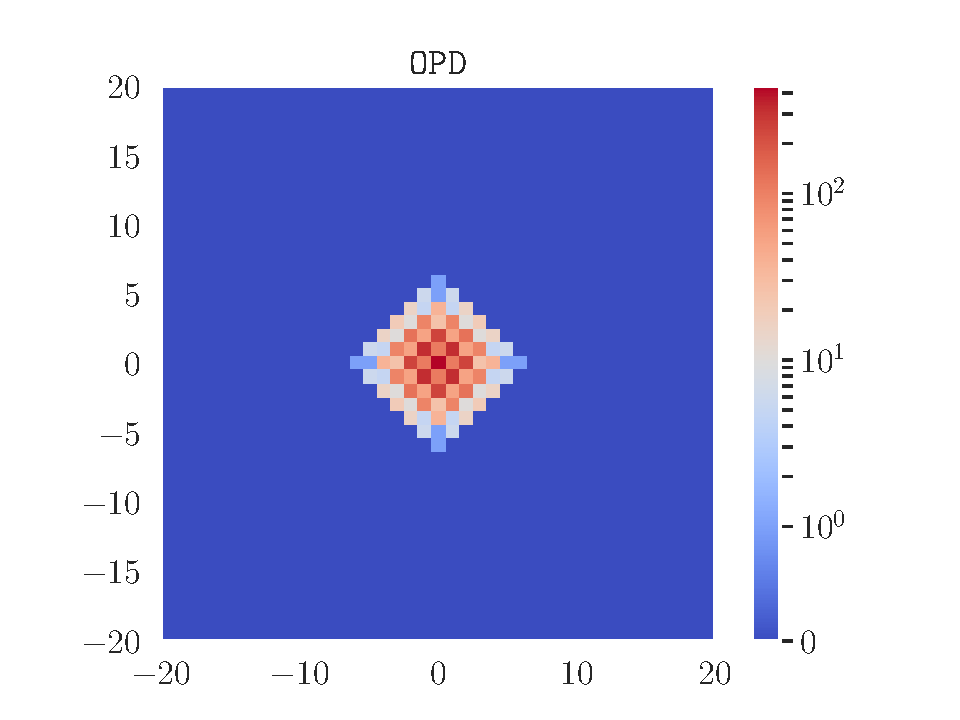
\includegraphics[width=0.6\linewidth]{../img/occupations_OPD}
	
	budget of $5460$ samples, maximum distance $d=6$
\end{center}
\end{itemize}
\end{alertblock}
\end{frame}

\begin{frame}{Goal}
\begin{exampleblock}{Better exploit this wasted information}
	\begin{itemize}
		\item<2-4> By \alert{merging} similar states \only<3>{into a {\green graph}}
	\end{itemize}
	\begin{center}
		\includegraphics<1>[trim={1.8cm 2.2cm 1.9cm 2.7cm}, clip, width=0.55\linewidth]{img/tree_simple}%
		\includegraphics<2>[trim={1.8cm 2.2cm 1.9cm 2.7cm}, clip, width=0.55\linewidth]{img/tree_merging}%
		\includegraphics<3>[trim={1.8cm 2.2cm 1.9cm 2.7cm}, clip, width=0.55\linewidth]{img/tree_merged}%
		\includegraphics<4>[trim={1.8cm 1.2cm 1.9cm 0.8cm}, clip, width=0.55\linewidth]{img/graph_simple}%
	\end{center}
\end{exampleblock}
\end{frame}

\begin{frame}{Questions}
\begin{center}
	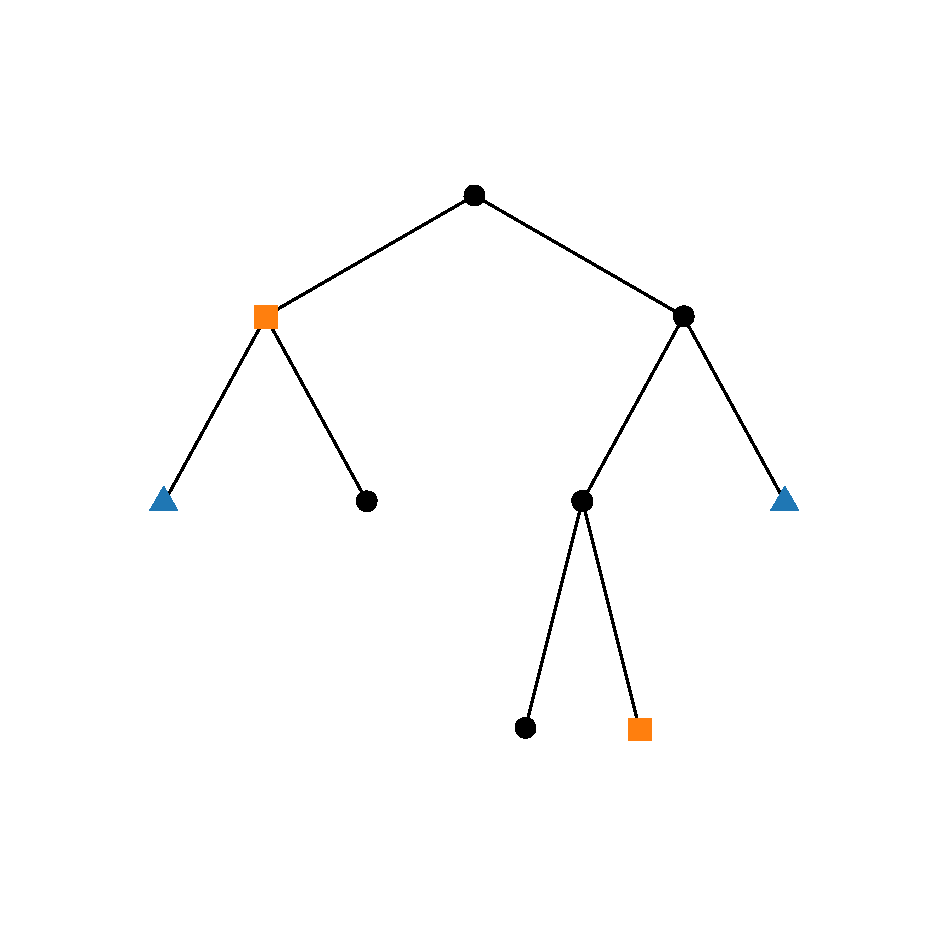
\includegraphics[trim={1.8cm 2.2cm 1.9cm 2.7cm}, clip,width=0.46\linewidth]{img/tree_simple}
	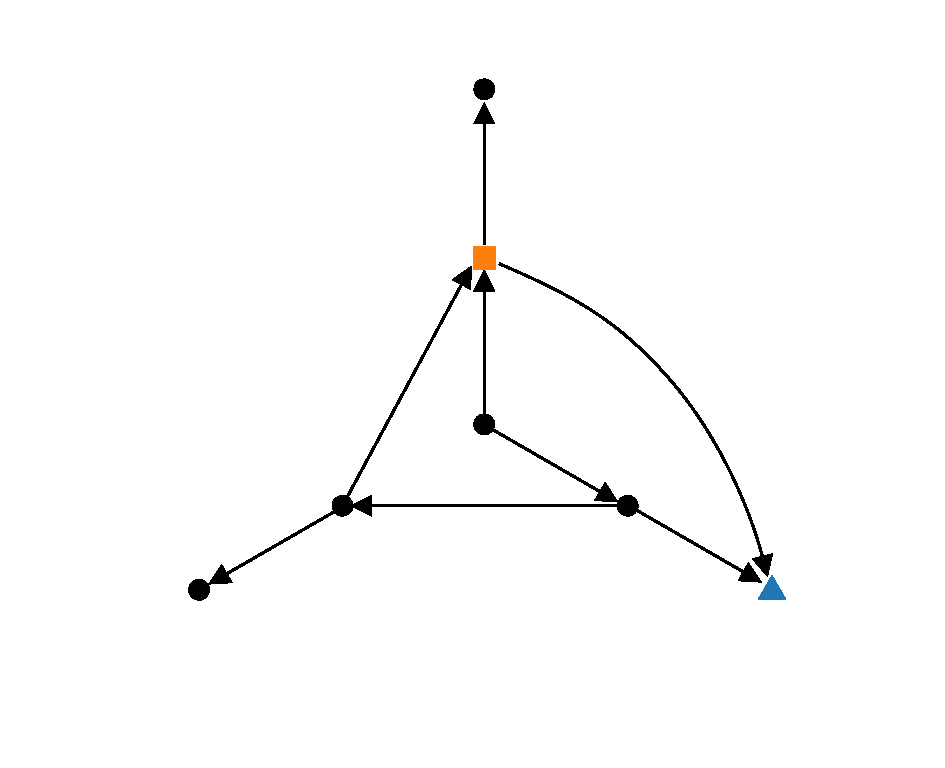
\includegraphics[trim={1.8cm 1.2cm 1.9cm 0.8cm}, clip,width=0.46\linewidth]{img/graph_simple}
\end{center}
\begin{itemize}
	\item How to \alert{adapt} MCTS algorithms to work on graphs?
	\item Can we \alert{quantify} the benefit of using graphs over trees?
\end{itemize}
\end{frame}

\begin{frame}{MCTS for Deterministic MDPs}
\begin{center}
	\includegraphics<1-3>[trim={1.8cm 1.5cm 1.9cm 2.7cm}, clip,width=0.35\linewidth]{../img/tree_1}%
	\includegraphics<4>[trim={1.8cm 1.5cm 1.9cm 2.7cm}, clip,width=0.35\linewidth]{img/tree_sample}%
	\includegraphics<5>[trim={1.8cm 1.5cm 1.9cm 2.7cm}, clip,width=0.35\linewidth]{img/tree_expand}%
\end{center}
\vspace*{-0.5cm}
\begin{block}{Optimism in the Face of Uncertainty: \texttt{OPD}}
\pause
\begin{enumerate}[<+->]
	\item Build \alert{confidence bounds} $L(a)\leq V(a) \leq U(a)$
	\item Follow \alert{optimistic} actions, from the root down to a leaf $b$
	\item \alert{Expand} the leaf $b\in\ext{T}_n$
\end{enumerate}
\end{block}
\end{frame}


\begin{frame}{On a graph...}

\begin{center}
	\includegraphics<1-2>[trim={1.0cm 0.8cm 1.9cm 0.8cm}, clip,width=0.35\linewidth]{../img/graph_1}%
	\includegraphics<3>[trim={1.0cm 0.8cm 1.9cm 0.8cm}, clip,width=0.35\linewidth]{img/graph_sample}%
	\includegraphics<4-6>[trim={0.8cm 0.8cm 1.9cm 0.8cm}, clip,width=0.35\linewidth]{img/graph_expand}%
\end{center}

\begin{block}{Same principle: \texttt{GBOP-D}}
	\pause
	\begin{enumerate}[<+->]
		\item Build \alert{confidence bounds} $L(s)\leq V(s) \leq U(s)$
		\item Follow \alert{optimistic} actions \textcolor<6>{red}{until an external node $s$ is reached}
		\item \alert{Expand} the external node $s\in\ext{\cG}_n$
		\begin{itemize}
			\item We are guaranteed to expand any state {\green only once}.
		\end{itemize}
	\end{enumerate}
\end{block}
\end{frame}

\begin{frame}{How to build the bounds $L,U$?}
How to bound $V(s) = \sup \sum_{t=0}^{\infty} \gamma^t r_t$?
\begin{itemize}[<+->]
	\item Initialize with trivial bounds:
	$\quad{\red L}=0,\quad {\orange U}=\frac{1}{1-\gamma}$
	\item Apply the Bellman operator ${\blue B}:V\to max_a R(s,a) + \gamma V(s')$
		$${\red L}(a) \leq {\blue B}({\red L})(a) \leq V(a) \leq {\blue B}({\orange U})(a) \leq {\orange U}(a)$$

	\item[] \begin{center}
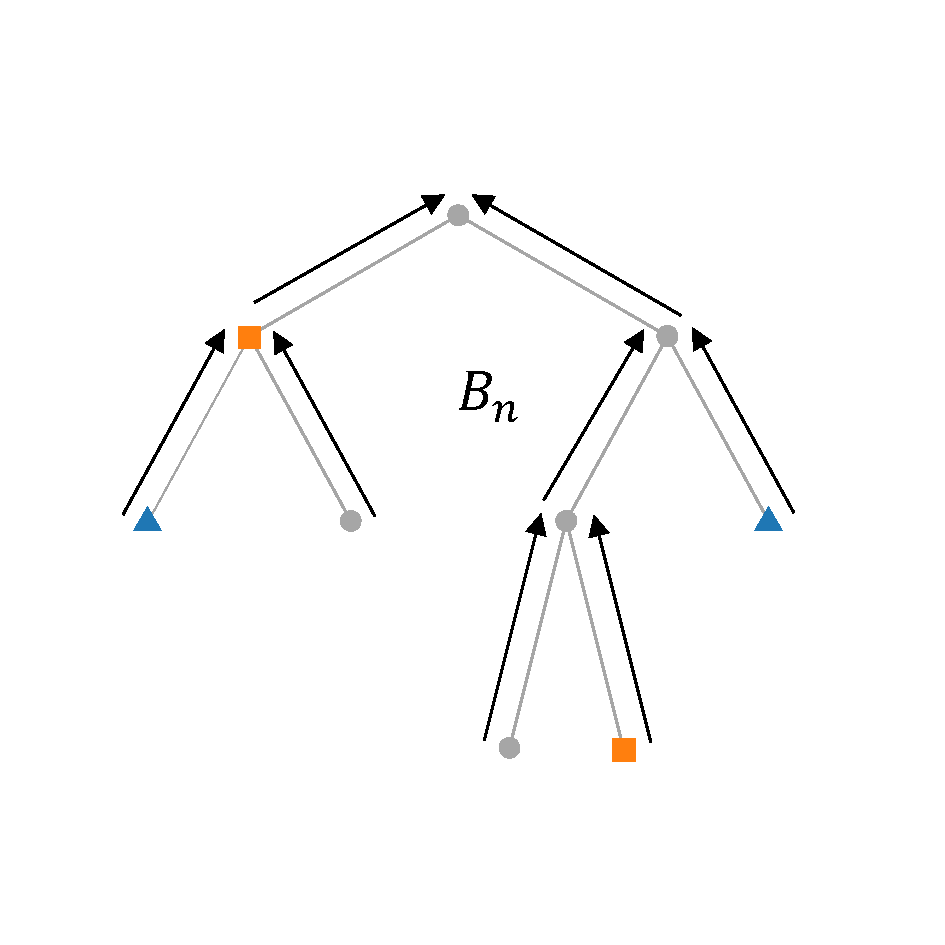
\includegraphics[trim={2.0cm 2.9cm 2.5cm 3.1cm}, clip,width=0.3\linewidth]{../img/tree_2}
\hspace*{1cm}
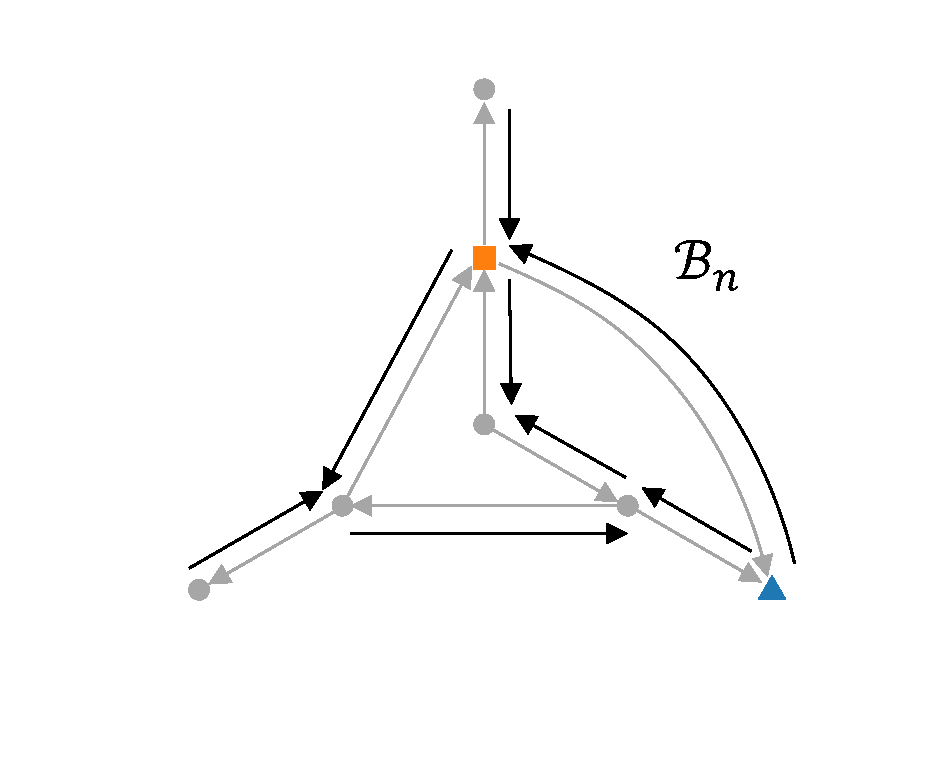
\includegraphics[trim={2.7cm 2.7cm 2.7cm 1.1cm}, clip,width=0.3\linewidth]{../img/graph_2}
	\end{center}
	\item \textbf{Trees}: Converges in {\green $d_n$ steps}
	\item \textbf{Graphs}: May converge in {\red $\infty$ steps} when there is a loop
\end{itemize}
\end{frame}

\begin{frame}{Analysis}
Is \texttt{GBOP-D} more efficient than \texttt{OPD}?

\pause
Performance: $r_n = V^\star - V(a_n)$
\pause
\begin{theorem}[Sample complexity of \texttt{OPD}, \cite{Hren2008optimistic}]
	\[r_n = \tilde{\cO}\left( n^{-\log \frac{1}{\gamma}/{\red \log\kappa}}\right),\]
	where ${\red \kappa}$ is a problem-dependent difficulty measure.
\end{theorem}
\pause
\begin{theorem}[Sample complexity of \texttt{GBOP-D}]
	\[r_n = \tilde{\cO}\left(n^{-\log \frac{1}{\gamma}/{\green \log \kappa_\infty}}\right),\]
	where ${\green \kappa_\infty}$ is a {\green tighter} problem-dependent difficulty measure:
	\[ {\green \kappa_\infty}\leq {\red \kappa} \]
\end{theorem}
\end{frame}

\begin{frame}{Comparing difficulty measures}
\begin{itemize}[<+->]
	\item ${\green \kappa_\infty} = {\red \kappa}$ if the MDP has a tree structure
	\item ${\green \kappa_\infty} < {\red \kappa}$ when trajectories intersect a lot
	\begin{itemize}
		\item actions cancel each-other out (e.g. moving left or right)
		\item actions are commutative (e.g. placing pawns on a board)
	\end{itemize}
\end{itemize}
\pause[\thebeamerpauses]
\begin{exampleblock}{Illustrative example: 3 states, $K>2$ actions}
	\begin{center}
    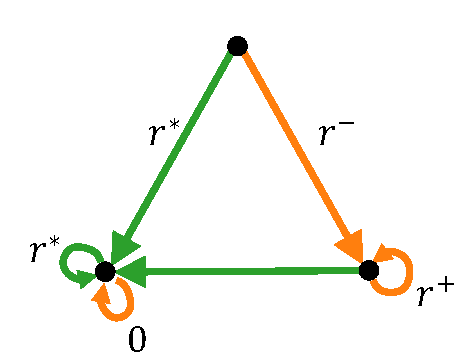
\includegraphics[trim={0.5cm 0.0cm 0.3cm 0.6cm}, clip, width=0.35\textwidth]{../img/mdp.pdf}
	\end{center}
	 $${\green \kappa_\infty = 1} < {\red \kappa = K-1}$$
\end{exampleblock}
\end{frame}

\begin{frame}{Experiment: sparse gridworld}
Rewards in a ball around $(10, 10)$ of radius $5$, with quadratic decay
\begin{center}
	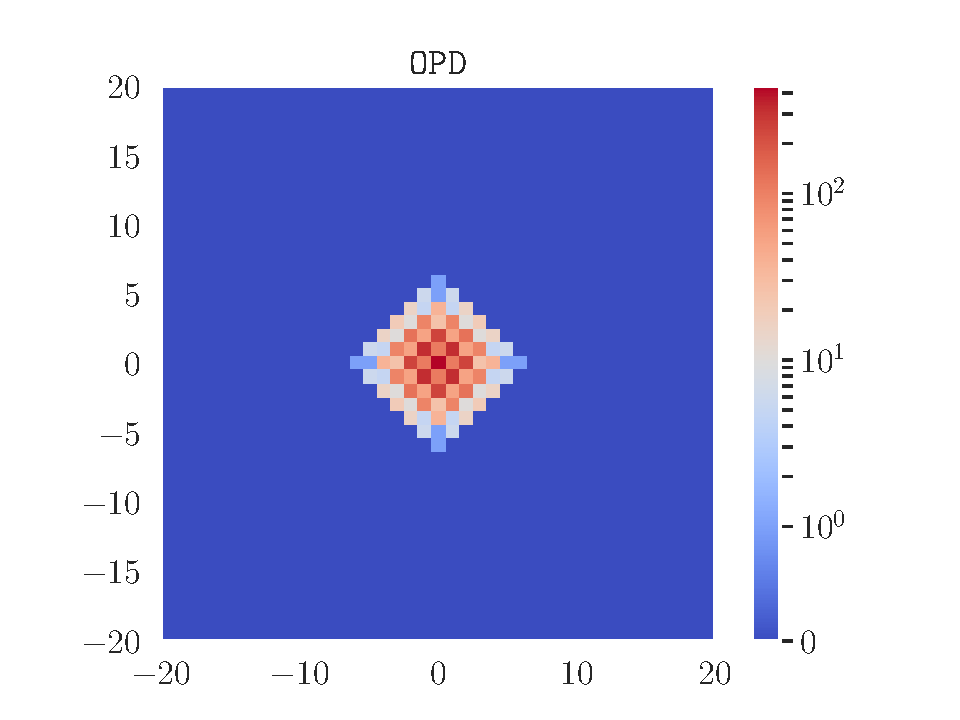
\includegraphics[trim={1.8cm 0.4cm 1.8cm 0.7cm}, clip, width=0.43\linewidth]{../img/occupations_OPD.pdf}
	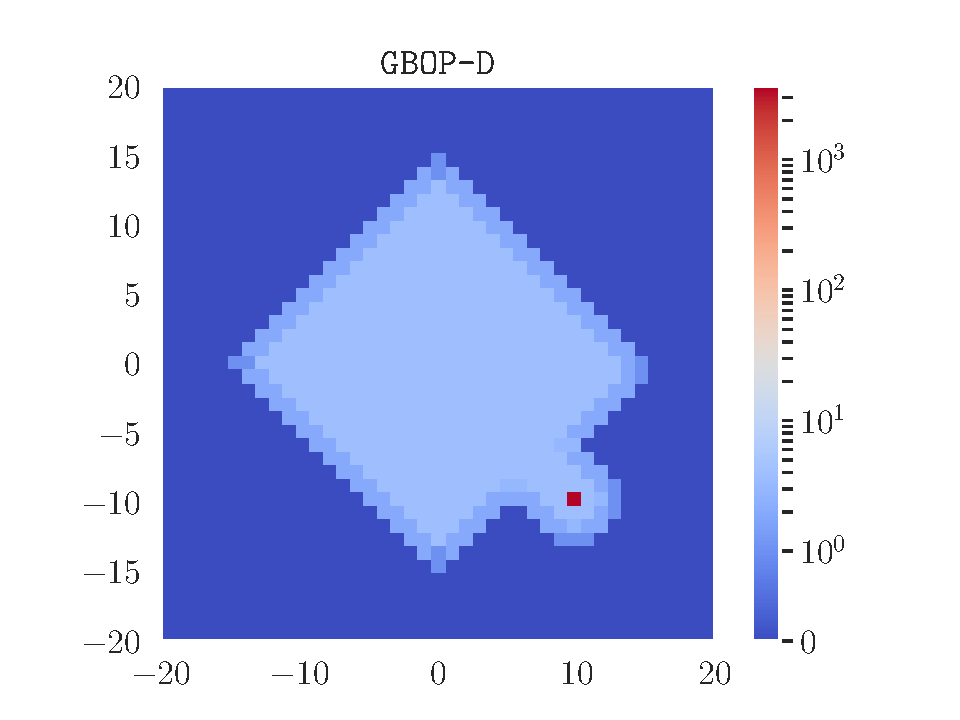
\includegraphics[trim={1.8cm 0.4cm 1.8cm 0.7cm}, clip, width=0.43\linewidth]{../img/occupations_GBOP-D.pdf}

	$n = 5640$ samples
\end{center}
\end{frame}

\begin{frame}{Extension to stochastic MDPs}
\begin{exampleblock}{Extension to stochastic MDPs}
\begin{itemize}
	\item Use state similarity to \alert{tighten} the bounds $L\leq V\leq U$.
	\item We adapt \texttt{MDP-GapE} (\cite{Jonsson2020planning}) to obtain \texttt{GBOP}
\end{itemize}
\end{exampleblock}
\end{frame}


\begin{frame}{Experiment: stochastic gridworld}
Noisy transitions with probability $p=10\%$
\begin{center}
	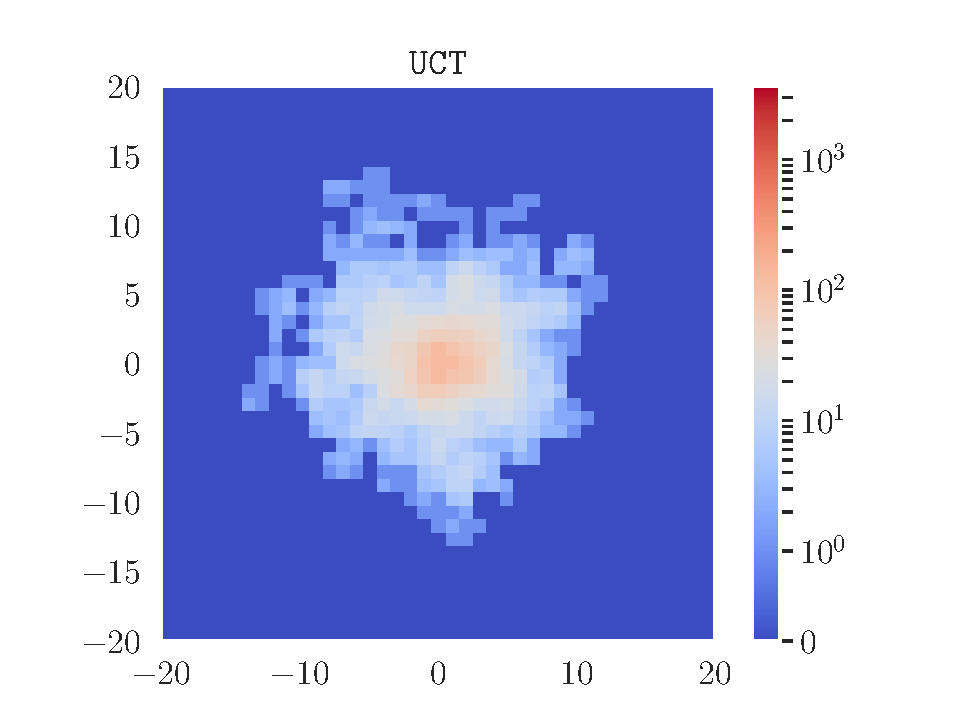
\includegraphics[trim={1.8cm 0.4cm 1.8cm 0.7cm}, clip, width=0.43\linewidth]{../img/occupations_UCT.pdf}
	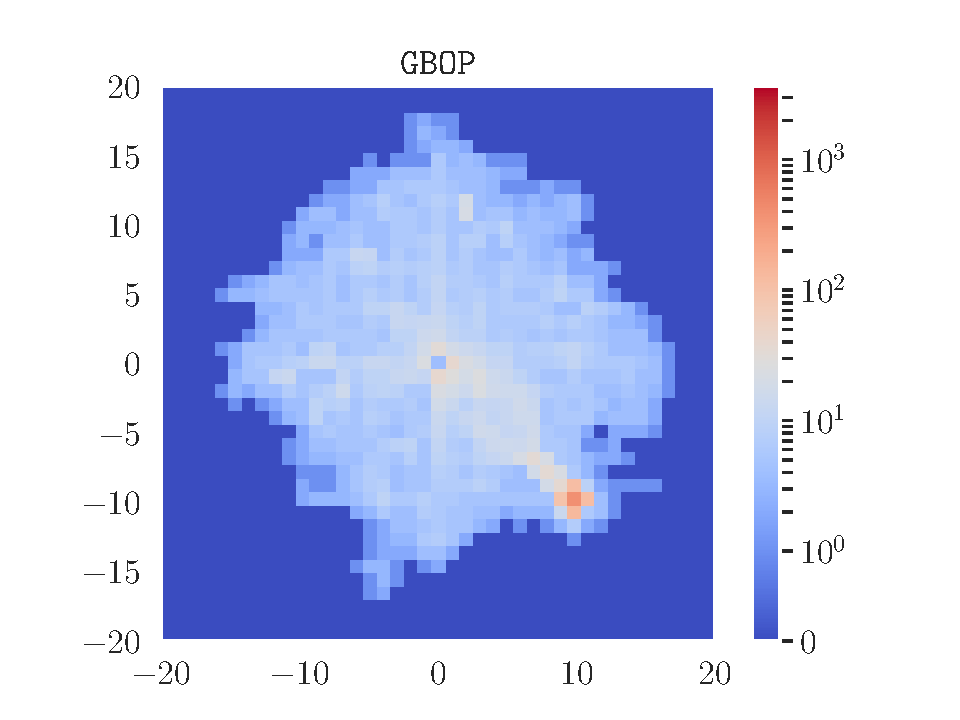
\includegraphics[trim={1.8cm 0.4cm 1.8cm 0.7cm}, clip, width=0.43\linewidth]{../img/occupations_GBOP.pdf}
	
	$n = 5640$ samples
\end{center}
\end{frame}

\begin{frame}{Exploration-Exploitation score}
$$S = \sum_{t=1}^n \underbrace{d(s_t, s_0)}_{\text{Exploration}} - \underbrace{d(s_t, s_g)}_{\text{Exploitation}}$$
\begin{center}
	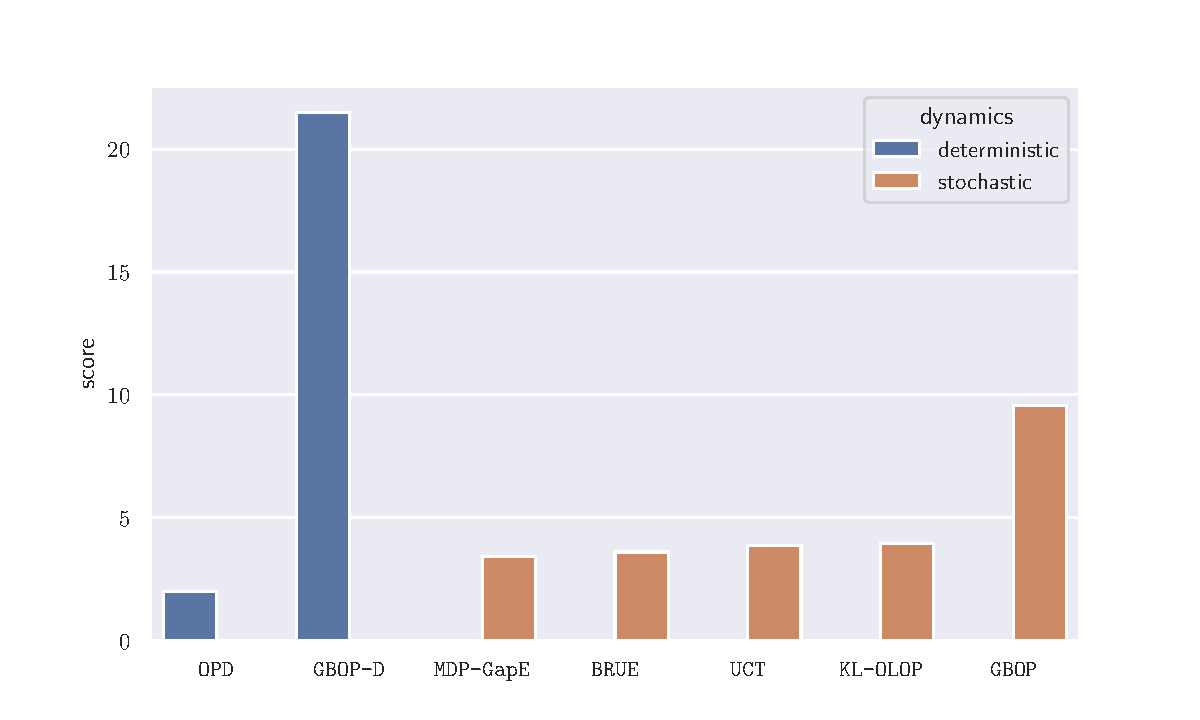
\includegraphics[trim = {1.4cm 0.cm 2cm 1.5cm}, clip, width=0.7\linewidth]{../img/score.pdf}

	$n = 5640$ samples
\end{center}
\end{frame}

\begin{frame}{Sailing Domain (\cite{Vanderbei1996})}
\begin{center}
	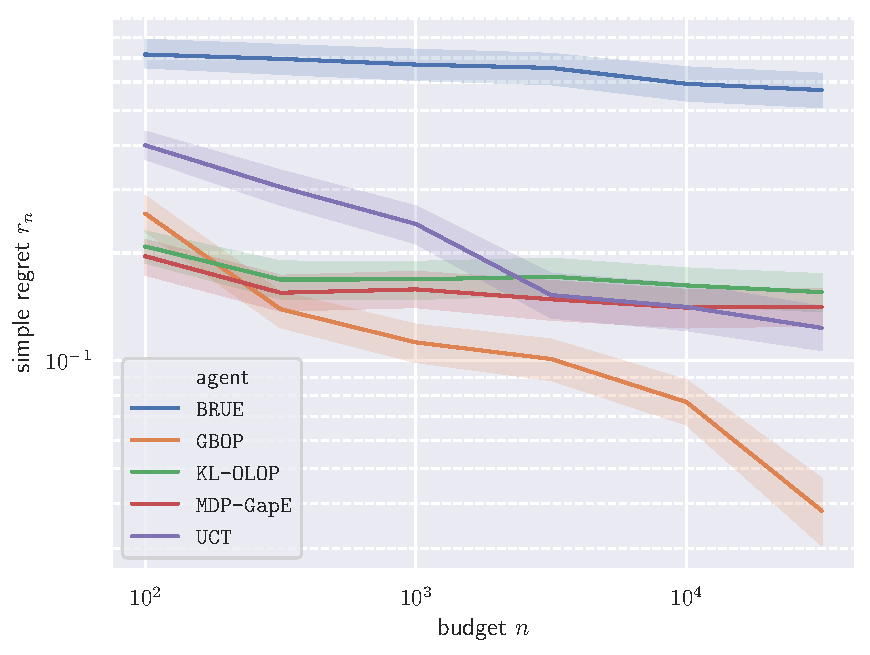
\includegraphics[trim = {0.2cm 0.2cm 0.7cm 0.5cm}, clip, width=0.6\linewidth]{../img/simple_regret.pdf}
\end{center}
\pause
\vspace*{-0.5cm}
Effective branching factor $\kappa_e$:
\begin{itemize}
	\item $\kappa_e \approx {\red 3.6}$, for \texttt{BRUE}, \texttt{KL-OLOP}, \texttt{MDP-GapE}, \texttt{UCT}
	\item $\kappa_e \approx {\green 1.2}$ for \texttt{GBOP}, which suggests our results may still hold
\end{itemize}
\end{frame}

\begin{frame}
\centering \LARGE Thank You!
\end{frame}


\end{document}
